%% When better models barely help: predictability limits in learned nonlinear robot control.
%% Every number is a macro from numbers.tex, generated by tools/fractal_numbers.py from results/fractal/.
\documentclass[conference]{IEEEtran}
\IEEEoverridecommandlockouts

\usepackage{cite}
\usepackage{amsmath,amssymb,amsfonts}
\usepackage{graphicx}
\usepackage{textcomp}
\usepackage{booktabs}
\usepackage{url}
\usepackage[hidelinks]{hyperref}

%% generated by tools/fractal_numbers.py -- do not edit by hand
\newcommand{\agreeCPU}{??}
\newcommand{\alphaAct}{0.25}
\newcommand{\alphaActC}{16.6}
\newcommand{\alphaActflip}{9.3\%}
\newcommand{\alphaActfloor}{2.2\%}
\newcommand{\alphaActhi}{0.31}
\newcommand{\alphaActlo}{0.20}
\newcommand{\alphaActn}{6}
\newcommand{\alphaCPU}{??}
\newcommand{\alphaCPUC}{??}
\newcommand{\alphaCPUflip}{??}
\newcommand{\alphaCPUfloor}{??}
\newcommand{\alphaCPUhi}{??}
\newcommand{\alphaCPUlo}{??}
\newcommand{\alphaCPUn}{??}
\newcommand{\alphaFine}{0.38}
\newcommand{\alphaFineC}{6.3}
\newcommand{\alphaFineflip}{2.2\%}
\newcommand{\alphaFinefloor}{0.8\%}
\newcommand{\alphaFinehi}{0.48}
\newcommand{\alphaFinelo}{0.30}
\newcommand{\alphaFinen}{5}
\newcommand{\alphaG}{0.28}
\newcommand{\alphaGC}{11.7}
\newcommand{\alphaGflip}{5.2\%}
\newcommand{\alphaGfloor}{0.3\%}
\newcommand{\alphaGhi}{0.35}
\newcommand{\alphaGlo}{0.23}
\newcommand{\alphaGn}{6}
\newcommand{\alphaICa}{0.28}
\newcommand{\alphaICaC}{11.7}
\newcommand{\alphaICaflip}{5.2\%}
\newcommand{\alphaICafloor}{0.3\%}
\newcommand{\alphaICahi}{0.35}
\newcommand{\alphaICalo}{0.23}
\newcommand{\alphaICan}{6}
\newcommand{\alphaICb}{0.29}
\newcommand{\alphaICbC}{11.2}
\newcommand{\alphaICbflip}{5.5\%}
\newcommand{\alphaICbfloor}{0.5\%}
\newcommand{\alphaICbhi}{0.36}
\newcommand{\alphaICblo}{0.23}
\newcommand{\alphaICbn}{6}
\newcommand{\alphaICc}{0.33}
\newcommand{\alphaICcC}{8.2}
\newcommand{\alphaICcflip}{4.8\%}
\newcommand{\alphaICcfloor}{0.7\%}
\newcommand{\alphaICchi}{0.41}
\newcommand{\alphaICclo}{0.27}
\newcommand{\alphaICcn}{6}
\newcommand{\alphaICd}{0.32}
\newcommand{\alphaICdC}{8.5}
\newcommand{\alphaICdflip}{4.7\%}
\newcommand{\alphaICdfloor}{0.7\%}
\newcommand{\alphaICdhi}{0.41}
\newcommand{\alphaICdlo}{0.27}
\newcommand{\alphaICdn}{6}
\newcommand{\alphaICe}{0.33}
\newcommand{\alphaICeC}{8.2}
\newcommand{\alphaICeflip}{5.5\%}
\newcommand{\alphaICefloor}{1.0\%}
\newcommand{\alphaICehi}{0.42}
\newcommand{\alphaICelo}{0.26}
\newcommand{\alphaICen}{6}
\newcommand{\alphaICmax}{0.33}
\newcommand{\alphaICmed}{0.32}
\newcommand{\alphaICmin}{0.28}
\newcommand{\alphaPol}{0.27}
\newcommand{\alphaPolC}{12.9}
\newcommand{\alphaPolflip}{7.2\%}
\newcommand{\alphaPolfloor}{0.3\%}
\newcommand{\alphaPolhi}{0.32}
\newcommand{\alphaPollo}{0.23}
\newcommand{\alphaPoln}{6}
\newcommand{\alphaState}{??}
\newcommand{\alphaStateC}{??}
\newcommand{\alphaStateflip}{0.0\%}
\newcommand{\alphaStatefloor}{0.0\%}
\newcommand{\alphaStatehi}{??}
\newcommand{\alphaStatelo}{??}
\newcommand{\alphaStaten}{0}
\newcommand{\alphaZoomOne}{0.04}
\newcommand{\alphaZoomOneC}{26171982.3}
\newcommand{\alphaZoomOneflip}{2.8\%}
\newcommand{\alphaZoomOnefloor}{0.5\%}
\newcommand{\alphaZoomOnehi}{0.16}
\newcommand{\alphaZoomOnelo}{-0.07}
\newcommand{\alphaZoomOnen}{5}
\newcommand{\alphaZoomTwo}{0.31}
\newcommand{\alphaZoomTwoC}{9.1}
\newcommand{\alphaZoomTwoflip}{10.5\%}
\newcommand{\alphaZoomTwofloor}{2.0\%}
\newcommand{\alphaZoomTwohi}{0.37}
\newcommand{\alphaZoomTwolo}{0.28}
\newcommand{\alphaZoomTwon}{6}
\newcommand{\bndAct}{31.0\%}
\newcommand{\bndGrid}{20.7\%}
\newcommand{\changeFine}{12.2\%}
\newcommand{\cpBnd}{2.9\%}
\newcommand{\divMilli}{10\%}
\newcommand{\divZero}{4\%}
\newcommand{\dzero}{2.3\%}
\newcommand{\icMechanism}{identical}
\newcommand{\lamHi}{2.4}
\newcommand{\lamLo}{1.4}
\newcommand{\nICbelow}{5}
\newcommand{\plateauFloor}{1.0\%}
\newcommand{\plateauHi}{2.8\%}
\newcommand{\plateauLo}{2.2\%}
\newcommand{\rzero}{0.0\%}
\newcommand{\stateHalf}{0.80}
\newcommand{\stateSucc}{99.9\%}
\newcommand{\succCPU}{??}
\newcommand{\succGrid}{20.5\%}
\newcommand{\tReach}{2.1}

\newcommand{\repo}{\url{https://github.com/anshM123/pendisacc}}

\begin{document}

\title{When Better Models Barely Help:\\
Predictability Limits in Learned Nonlinear Robot Control}

\author{\IEEEauthorblockN{Amitosh Mishra}
\IEEEauthorblockA{\textit{Independent Researcher}\\
amitosh.mishra81@gmail.com}}

\maketitle

\begin{abstract}
Sim-to-real practice assumes that a more accurate model buys proportionally more
certainty about whether a policy will work. We measure that payoff directly.
For a frozen reinforcement-learning swing-up controller on a triple inverted
pendulum we sample pairs of simulators that differ by a perturbation of size
$\epsilon$. We record how often one member of a pair
succeeds and the other fails. Over the resolved range this outcome-flip
probability falls only as $\epsilon^{\alpha}$ with $\alpha=\alphaG$
($95\%$ CI $[\alphaGlo,\alphaGhi]$), where a smooth success boundary would give
$\alpha=1$. The consequence is concrete: halving the chance of mispredicting the
outcome requires about $\alphaGC\times$ tighter model accuracy. At $0.1\%$
mass precision, $\alphaGflip$ of perturbation pairs still disagree. The exponent
reproduces across a second policy ($\alphaPol$), a mass--actuator-lag
plane ($\alphaAct$), a zoom on the main boundary ($\alphaZoomTwo$), five initial
conditions (median $\alphaICmed$), an independent non-PhysX dynamics implementation
($\alphaCPU$), and a halved physics step ($\alphaFine$). By contrast, the same policy
is almost insensitive to its initial state: $\stateSucc$ success over $\pm0.8$\,rad of
initial link offsets. The unpredictability lives in the model, not the start. Outcome-divergent trajectories
separate at $\lamLo$--$\lamHi$\,s$^{-1}$, which explains a floor set by
the simulator's own numerical precision. Every test was pre-registered before it
ran. A registered zoom onto an isolated success island failed, and we report it.
All results are in simulation. Code, pre-registrations and raw data: \repo.
\end{abstract}

\begin{IEEEkeywords}
sim-to-real transfer, predictability, nonlinear dynamics, reinforcement learning, underactuated robots
\end{IEEEkeywords}

\begin{figure*}[t]
\centering
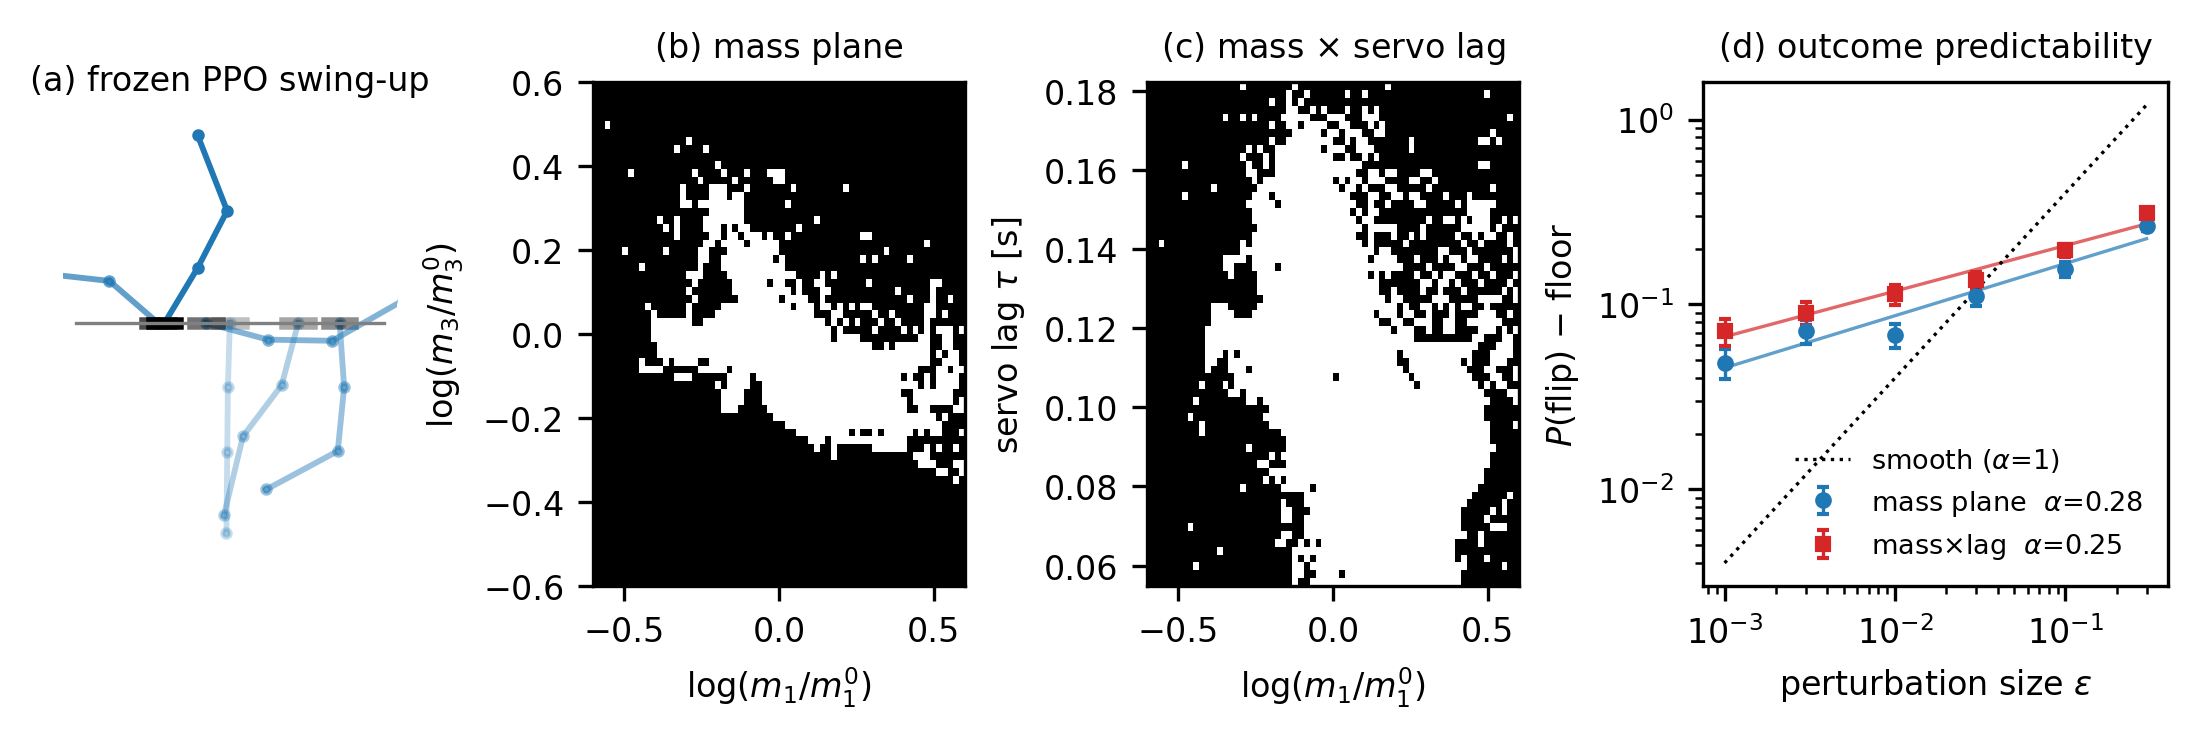
\includegraphics[width=\textwidth]{../figures/fig_pred_main.png}
\caption{\textbf{Outcome predictability of a learned controller.}
(a)~Triple inverted pendulum on a velocity-servoed cart; one frozen PPO swing-up policy.
(b)~Success (white) over link-1 and link-3 mass, from one fixed initial condition.
(c)~Success over link-1 mass and servo lag.
(d)~Probability that two simulators a distance $\epsilon$ apart disagree on the outcome, with the
same-parameter noise floor subtracted. A smooth boundary gives slope $1$ (dotted); the measured
slopes are $\alphaG$ and $\alphaAct$, so a $10\times$ better model removes only
$1-10^{-\alpha}\approx 48\%$ of outcome ambiguity.}
\label{fig:main}
\end{figure*}

\section{Introduction}
Two kinds of work treat modelling error as a quantity to shrink: system identification and
the calibration side of domain randomisation~\cite{tobin2017,peng2018}. Both implicitly assume that the
payoff is roughly proportional: halve the parameter error and the chance of being wrong
about whether the robot succeeds should roughly halve. We ask how true that is for a
learned controller on a strongly nonlinear robot. We measure the payoff instead of assuming it.

The tool is old. For dynamical systems with competing outcomes, Grebogi \emph{et al.}\ defined
the \emph{uncertainty exponent}: the fraction of initial conditions whose final state changes
under a perturbation of size $\epsilon$ scales as $\epsilon^{\alpha}$~\cite{grebogi1983,mcdonald1985}.
$\alpha=1$ for a smooth boundary. $\alpha<1$ means predictability improves slowly with
precision. We apply this measure to a quantity robotics cares about, whether a deployed
learned policy \emph{succeeds}, in the space robotics actually calibrates: simulator
parameters.

On a triple inverted pendulum swing-up controlled by a frozen PPO policy, the answer is
$\alpha\approx\alphaG$ over two and a half decades of $\epsilon$. A $10\times$ better model removes
less than half of the ambiguity about the outcome. Contributions:
\begin{enumerate}
\item \textbf{An empirical law} relating model uncertainty to outcome uncertainty for a
learned controller, with a direct engineering translation: $C_{1/2}=2^{1/\alpha}$, the precision
gain needed to halve outcome ambiguity.
\item \textbf{Pre-registered replication} across policies, physical and actuator uncertainty,
initial conditions, an independent dynamics implementation and numerical resolution. A contrasting
null in initial-state space and the registered failures are reported.
\item \textbf{A mechanism}: finite-time amplification along outcome-divergent trajectories, which
also sets a numerical floor below which a simulator cannot resolve transfer at all.
\item \textbf{Measurement practice}: $f(\epsilon)$ is cheap to measure with vectorised simulation and
should precede investment in model accuracy.
\end{enumerate}

\section{Related Work}
\emph{Final-state sensitivity.} Fractal and rough basin boundaries, and the uncertainty exponent
that quantifies them, are classical in nonlinear dynamics~\cite{grebogi1983,mcdonald1985}.
Robotics has found fractal basins of attraction in \emph{state} space for running
models~\cite{cnops2015}. We do not claim that rough boundaries in state space are new.

\emph{Rough structure in learning.} Wang \emph{et al.}\ show that policy-optimisation objectives can be
fractal as functions of \emph{policy} parameters, which obstructs gradient
estimation~\cite{wang2023}. Sohl-Dickstein finds fractal trainability boundaries in
\emph{hyperparameter} space~\cite{sohldickstein2024}. Our object differs. We hold the policy fixed and ask
about the success boundary over \emph{simulator} parameters, the axes along which sim-to-real transfer
is calibrated.

\emph{Sim-to-real.} Domain randomisation~\cite{tobin2017,peng2018} widens the training distribution, and
system identification narrows the model error~\cite{gautier1990}. Neither literature, to our knowledge,
measures how the \emph{outcome} of a fixed policy becomes predictable as model error shrinks. In an
earlier study of the same robot, mass \emph{ratios} dominated transfer while overall scale was irrelevant,
consistent with dimensional similarity~\cite{girard2024,pascoa2025}. Here we look at the geometry of the
boundary itself.

\section{System and Protocol}\label{sec:setup}
\emph{Robot and policy.} A cart on a $\pm0.6$\,m rail carries three passive links. The corrected CAD model
has steel shaft links and PETG arms. The cart is driven through a first-order velocity servo
($\tau=0.1$\,s, loop gain $400$\,N\,s/m, $349.5$\,N clamp) at $250$\,Hz in Isaac Lab. Swing-up
policies are trained with PPO (4096 environments, 1000 iterations) and then frozen. Policy A
(\texttt{CORR\_s1}) is primary; policy B (\texttt{T5\_orbit\_s1}) was trained independently.

\emph{Success.} An episode (12\,s, starting hanging) succeeds if the cart never leaves the rail, the tip
reaches upright ($>0.9$ of full height), and the tip is upright for more than $95\%$ of the final quarter.

\emph{Determinism.} The stock task randomises the initial state, which would make any map speckled for
reasons unrelated to the boundary. Every environment therefore starts from one fixed state, set through a
per-environment initial-condition table. Re-running a full map in a new process reproduces all outcomes
($\rzero$ disagreement). Routing the initial condition through the table reproduced the original run on
all $8400$ environments (\icMechanism).

\emph{Pre-registration.} Every test, window, threshold and decision rule was committed to the
repository before the run it governs (\texttt{PREREGISTRATION\_FRACTAL.md}). Addenda record results and
any new test in commit order.

\section{Measuring Outcome Predictability}\label{sec:method}
Let $S(\theta)\in\{0,1\}$ be the outcome of the frozen policy in the simulator with parameters
$\theta$ (log-scale factors), or from initial state $\theta$. We draw $600$ base points uniformly in a
window. Each is paired with $\theta+\epsilon u$, where $u$ is a random unit vector, for
$\epsilon\in\{0.3,0.1,0.03,0.01,0.003,0.001\}$. We record
\begin{equation}
f(\epsilon)=\Pr\big[S(\theta)\neq S(\theta+\epsilon u)\big].
\end{equation}
Pairs at $\epsilon=0$, identical parameters in different environment slots, give a noise floor $f_0$.
The usable scales are those with $f(\epsilon)-f_0$ at least three standard errors above zero. $\alpha$ is
the least-squares slope of $\log(f-f_0)$ against $\log\epsilon$ over those scales, with a $95\%$
bootstrap interval over pairs. A smooth, finite-length boundary gives $f\propto\epsilon$, i.e.\
$\alpha=1$~\cite{mcdonald1985}. The engineering reading is
\begin{equation}
C_{1/2}=2^{1/\alpha},
\end{equation}
the factor by which $\epsilon$ must shrink to halve $f$. It is valid only over the resolved range of
$\epsilon$.

Two controls guard the estimate. A flip whose two episodes both sit within $0.05$ of the hold threshold
is counted as \emph{threshold jitter}. At most $3\%$ of flips were of that kind. Every exponent is reported
with its number of usable scales.

We do not call the boundary fractal. The resolved range is about $2.5$ decades, bounded below by
simulator precision (Sec.~\ref{sec:floor}), and one registered zoom test failed.

\section{Results}\label{sec:results}

\subsection{A rough transfer boundary}
On the $m_1\times m_3$ plane (window $\pm0.6$ in log scale), policy A succeeds on $\succGrid$ of a
$64\times64$ grid. The success region is a band: heavier link~1 must be offset by lighter link~3.
$\bndGrid$ of cells border a cell with the opposite outcome (Fig.~\ref{fig:main}b). Pair sampling gives
$\alpha=\alphaG$ over $\alphaGn$ usable scales, and $f(10^{-3})=\alphaGflip$ against a floor of
$\alphaGfloor$ (Fig.~\ref{fig:main}d). A model accurate to $0.1\%$ in two link masses still leaves the
outcome unresolved for about one base point in twenty.

\subsection{Replication}
Table~\ref{tab:repl} collects every registered exponent; Fig.~\ref{fig:repl} shows the curves.

\emph{Policy.} Independently trained policy B gives $\alphaPol$ $[\alphaPollo,\alphaPolhi]$.

\emph{Uncertainty family.} Replacing $m_3$ by the servo time constant, an actuator property, gives
$\alphaAct$ $[\alphaActlo,\alphaActhi]$ with $f(10^{-3})=\alphaActflip$. So the roughness is not specific to mass.

\emph{Initial conditions.} Five fixed initial conditions spanning the task's initialisation range give
median $\alpha=\alphaICmed$ (range $\alphaICmin$--$\alphaICmax$). $\nICbelow$ of $5$ are below $0.8$.

\emph{Dynamics implementation.} The same policy and the same $4200$ parameter pairs, run in an independent
analytical model (explicit integration, no PhysX), give $\alpha=\alphaCPU$ $[\alphaCPUlo,\alphaCPUhi]$.
Isaac and the analytical model agree on $\agreeCPU$ of individual outcomes.

\emph{Resolution.} Halving the physics step at a fixed $250$\,Hz control rate gives $\alphaFine$
$[\alphaFinelo,\alphaFinehi]$, with floor $\alphaFinefloor$.

\emph{Initial state (contrast).} Holding the physics nominal, we perturbed the initial angles of link~1
and joint~2. The registered rule widened the window from $\pm0.05$ to $\pm0.2$ and then $\pm0.8$\,rad while
success stayed above $98\%$. At $\pm0.8$\,rad it was still $\stateSucc$, so the test is uninformative on
$\alpha$. There is almost no boundary to measure. The swing-up funnels a wide range of starting states
into success, while tiny changes to the plant decide it.

\emph{Zoom.} The registered zoom was centred on the grid cell with the most disagreeing neighbours. That cell
was an isolated success island, where base success is $1$--$2\%$ and outcomes flip at the same rate at
every scale ($\alpha=\alphaZoomOne$). It failed its criterion. A second zoom, registered after that result
and centred on the main success boundary, gives $\alphaZoomTwo$. The honest statement is that the
exponent reproduces at the main boundary. Isolated islands behave like independent coin flips.

\begin{table}[t]
\caption{Pre-registered uncertainty exponents (bootstrap 95\% CI). $n$: usable scales.
$C_{1/2}=2^{1/\alpha}$: precision gain needed to halve outcome ambiguity.}
\label{tab:repl}
\centering\footnotesize
\setlength{\tabcolsep}{3pt}
\begin{tabular}{@{}llccc@{}}
\toprule
Test & Plane / condition & $\alpha$ [95\% CI] & $n$ & $C_{1/2}$\\
\midrule
Primary (Isaac)       & $m_1\times m_3$, policy A & $\alphaG$ [$\alphaGlo$, $\alphaGhi$] & $\alphaGn$ & $\alphaGC$\\
Second policy         & $m_1\times m_3$, policy B & $\alphaPol$ [$\alphaPollo$, $\alphaPolhi$] & $\alphaPoln$ & $\alphaPolC$\\
Actuator plane        & $m_1\times\tau$           & $\alphaAct$ [$\alphaActlo$, $\alphaActhi$] & $\alphaActn$ & $\alphaActC$\\
Zoom, main boundary   & $\pm0.06$ window          & $\alphaZoomTwo$ [$\alphaZoomTwolo$, $\alphaZoomTwohi$] & $\alphaZoomTwon$ & $\alphaZoomTwoC$\\
Zoom, isolated island & \textbf{failed}           & $\alphaZoomOne$ & $\alphaZoomOnen$ & --\\
Independent dynamics  & analytical, no PhysX      & $\alphaCPU$ [$\alphaCPUlo$, $\alphaCPUhi$] & $\alphaCPUn$ & $\alphaCPUC$\\
Resolution            & physics d$t/2$            & $\alphaFine$ [$\alphaFinelo$, $\alphaFinehi$] & $\alphaFinen$ & $\alphaFineC$\\
Initial state         & $\pm0.8$\,rad, nominal plant & \multicolumn{3}{c}{uninformative: $\stateSucc$ success}\\
IC 0--4               & $m_1\times m_3$           & \multicolumn{3}{c}{$\alphaICa$, $\alphaICb$, $\alphaICc$, $\alphaICd$, $\alphaICe$}\\
\bottomrule
\end{tabular}
\end{table}

\begin{figure*}[t]
\centering
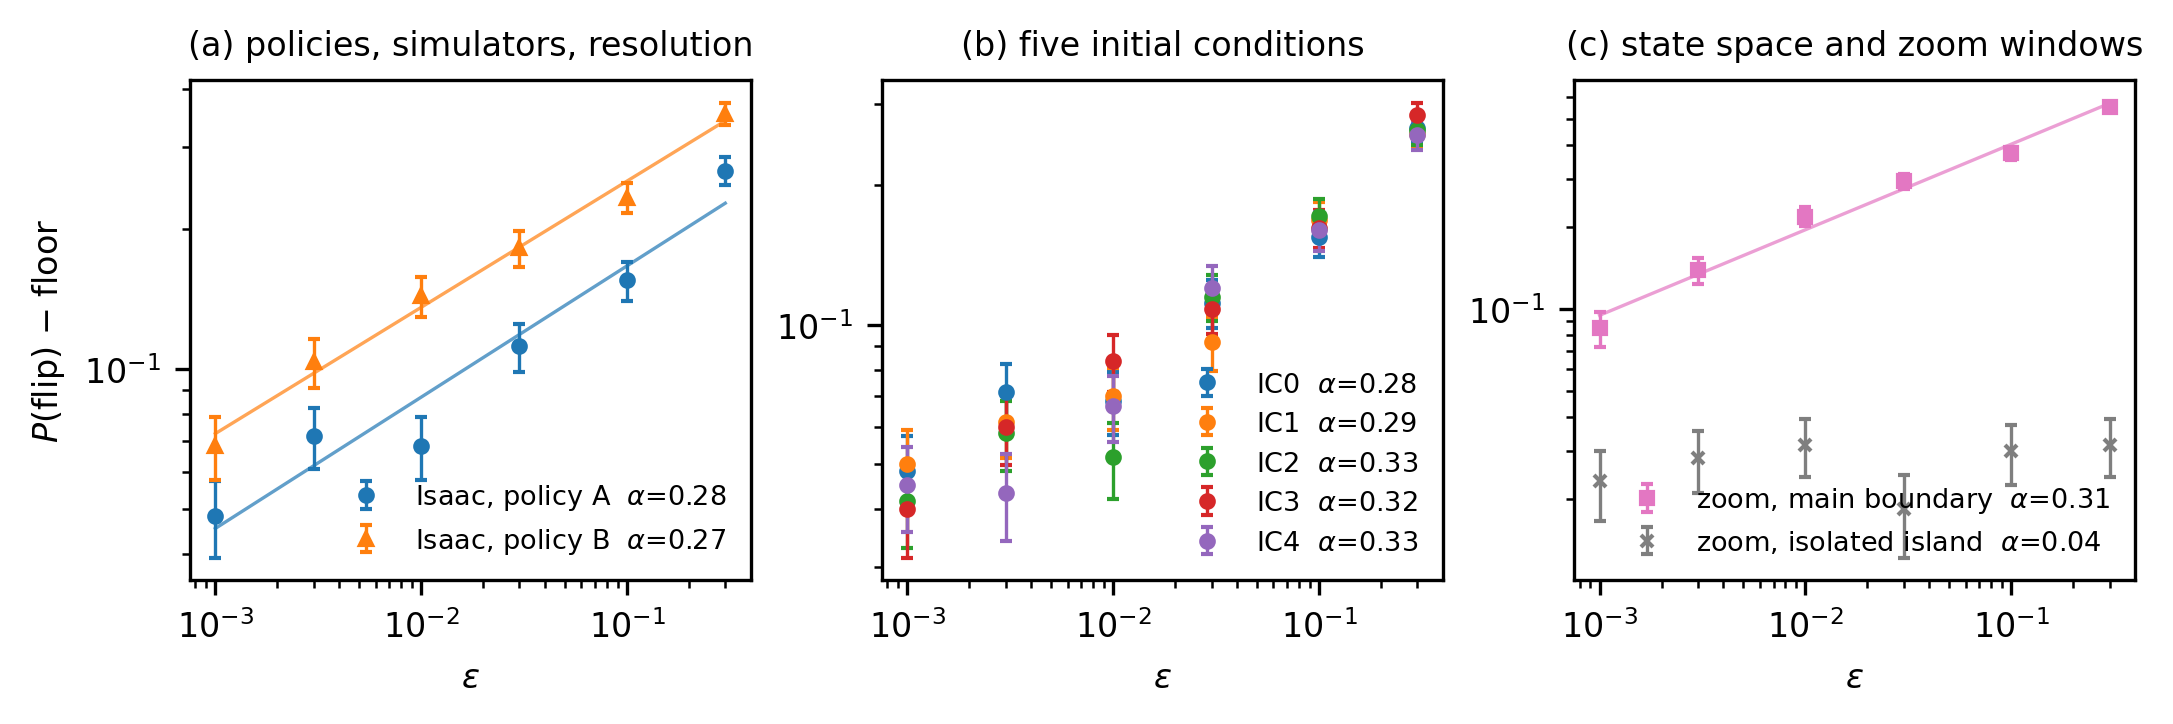
\includegraphics[width=\textwidth]{../figures/fig_pred_repl.png}
\caption{\textbf{Replication.} Floor-subtracted flip probability with fits over usable scales.
(a)~Second policy, independent analytical dynamics, and halved physics step.
(b)~Five fixed initial conditions.
(c)~Zoom on the main boundary, and the failed zoom on an isolated island, which is flat.}
\label{fig:repl}
\end{figure*}

\subsection{Resolved range and numerical floor}\label{sec:floor}
Below $\epsilon\approx3\times10^{-4}$, $f$ stops falling and levels off at $\plateauLo$--$\plateauHi$
against a same-parameter floor of $\plateauFloor$ (Fig.~\ref{fig:mech}b). Identical parameters placed
in different environment slots of one batch disagree on $\dzero$ of grid cells. The simulator is
deterministic run to run, so this is sensitivity to slot-dependent floating-point differences.
Transfer is not resolvable below that scale in this simulator.

\subsection{Mechanism: finite-time amplification}
Twin episodes differing by $\epsilon$ in link-1 mass were recorded in full. Most twins stay close,
because most parameter points lie deep inside one outcome region. The twins that end far apart ($\divMilli$
at $\epsilon=10^{-3}$, $\divZero$ even at $\epsilon=0$) separate exponentially at
$\lamLo$--$\lamHi$\,s$^{-1}$ and reach $0.1$ in about $\tReach$\,s (Fig.~\ref{fig:mech}a). Over a
12\,s episode that amplifies solver-level differences to order one, which accounts for the floor. We
report this as finite-time amplification. It is not a proof of chaos.

\subsection{Contrast system}
The stock Isaac Lab cartpole, trained and frozen the same way, has a sparse, clean boundary. Only
$\cpBnd$ of cells border the opposite outcome, there are no isolated islands, and no pair flipped for
$\epsilon\le0.01$ (Fig.~\ref{fig:mech}c). Too few flips were resolved to estimate its exponent, so the
comparison is qualitative only.

\begin{figure*}[t]
\centering
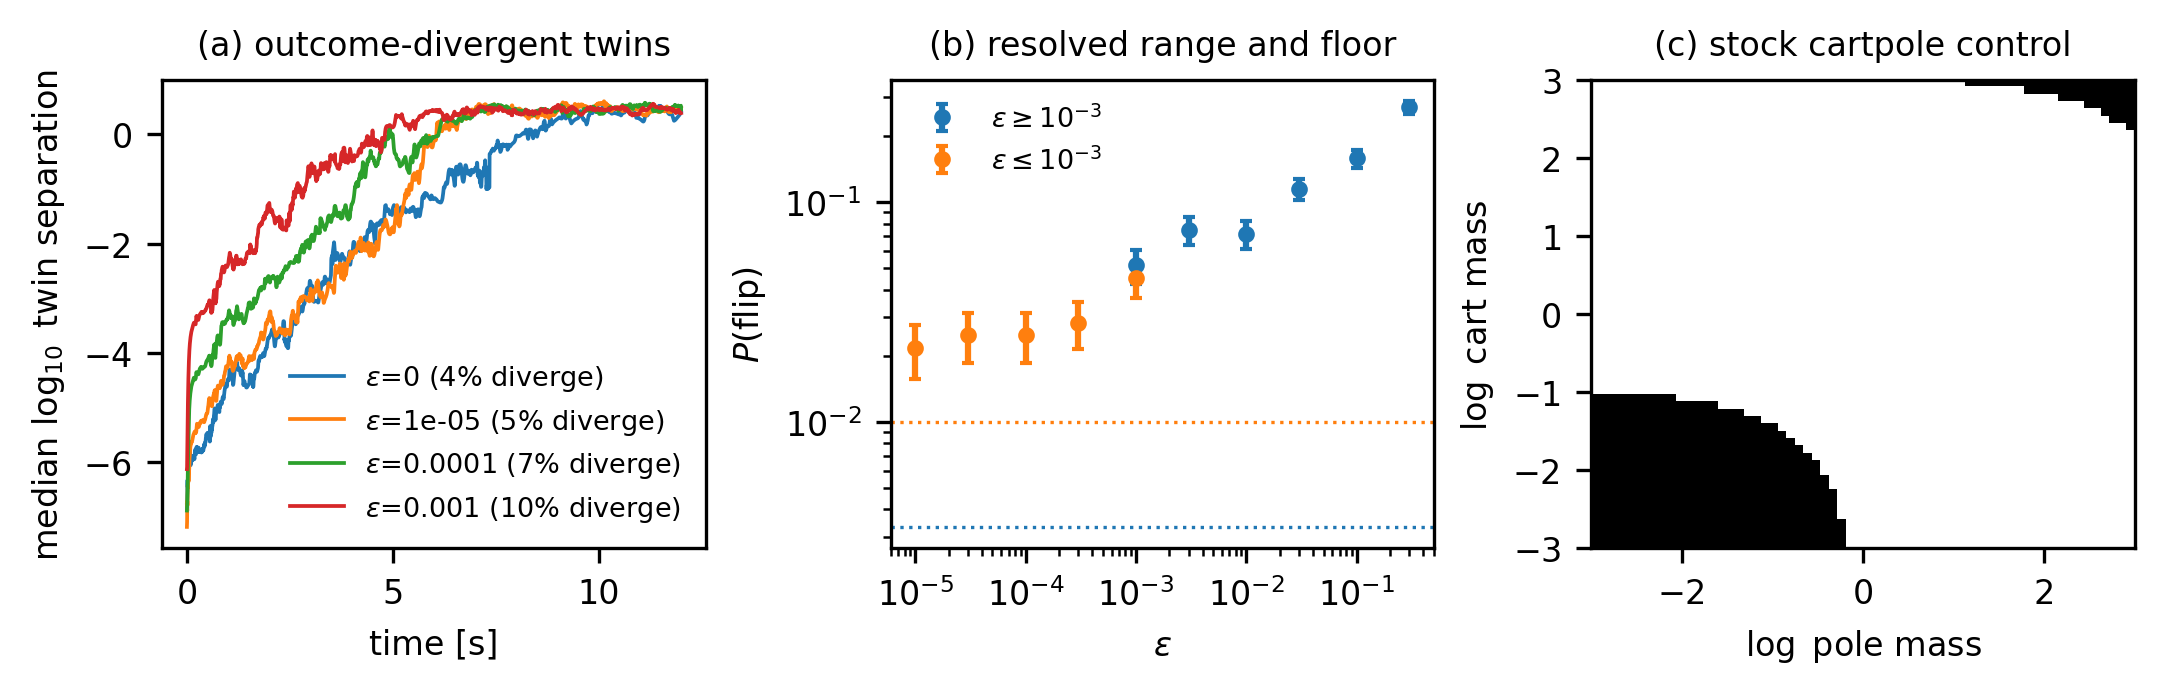
\includegraphics[width=\textwidth]{../figures/fig_pred_mech.png}
\caption{\textbf{Mechanism and limits.} (a)~Median separation of outcome-divergent twin episodes.
(b)~Flip probability down to $\epsilon=10^{-5}$: the power law ends at the simulator's own floor (dotted).
(c)~Stock cartpole: a clean boundary.}
\label{fig:mech}
\end{figure*}

\section{Consequences}
\emph{For calibration.} With $\alpha\approx0.25$--$0.32$, halving the probability of a wrong
transfer prediction near the boundary needs about $9$--$16\times$ better parameter accuracy, and a $10\times$
improvement removes less than half the ambiguity. Identification effort can therefore have sharply
diminishing returns, not because the model stays wrong but because the outcome is intrinsically hard to
predict near the boundary.

\emph{Model versus state.} For this task the ambiguity is concentrated in the plant, not the start. The
policy tolerates large initial-state errors but not $0.1\%$ model errors near the boundary. Effort spent on
state estimation at the start would be wasted, and effort on model accuracy pays off slowly.

\emph{For practice.} $f(\epsilon)$ is cheap to measure: one vectorised run of a few thousand
environments. It can tell a practitioner whether to invest in model accuracy or in moving the policy's
operating point away from the boundary (robustness margin). The same machinery also exposes the
simulator's resolution limit for a given task.

\section{Limitations and What Failed}
\emph{Scope.} One robot and one task family, with two policies, all in simulation. The hardware is under
construction, and nothing here has been tested on it. The resolved range is $2.5$ decades, so the power
law must not be extrapolated beyond it. $C_{1/2}$ describes the near-boundary regime sampled by the
windows used here.

\emph{Registered failures.} The first zoom test failed (Sec.~\ref{sec:results}). The cartpole control was
uninformative on $\alpha$. Before this study, a pre-registered screen of $54$ hypotheses about predicting
transfer from local stability quantities was run on the same robot. Its leads failed replication on fresh
Isaac data. For example, a closed-loop damping predictor had Spearman $0.69$ on $24$ old policies and $0.07$
on the fresh data. That failure is consistent with the present finding: a smooth, local predictor of a
rough outcome boundary should not generalise.

\emph{Novelty.} Rough and fractal basins in state space and fractal structure in learning landscapes are
known~\cite{grebogi1983,mcdonald1985,cnops2015,wang2023,sohldickstein2024}. Our claim is narrow: we measure
the outcome-predictability exponent of a \emph{fixed learned controller} over \emph{simulator parameters},
show that it replicates, and translate it into what calibration can and cannot buy.

\section{Conclusion}
For a learned controller on a strongly nonlinear robot, the probability of mispredicting success falls
only as $\epsilon^{\alphaG}$ with model error over the resolved range. Better models barely help near the
boundary. The measurement costs one vectorised simulation run, and it should be taken before assuming
that accuracy will pay off.

\begin{thebibliography}{00}
\bibitem{tobin2017} J. Tobin \emph{et al.}, ``Domain randomization for
transferring deep neural networks from simulation to the real world,'' in
\emph{IROS}, 2017.
\bibitem{peng2018} X. B. Peng \emph{et al.}, ``Sim-to-real transfer of robotic
control with dynamics randomization,'' in \emph{ICRA}, 2018.
\bibitem{grebogi1983} C. Grebogi, S. W. McDonald, E. Ott and J. A. Yorke, ``Final state sensitivity: an
obstruction to predictability,'' \emph{Phys. Lett. A}, vol. 99, no. 9, pp. 415--418, 1983.
\bibitem{mcdonald1985} S. W. McDonald, C. Grebogi, E. Ott and J. A. Yorke, ``Fractal basin boundaries,''
\emph{Physica D}, vol. 17, no. 2, pp. 125--153, 1985.
\bibitem{cnops2015} T. Cnops, Z. Gan and C. D. Remy, ``The basin of attraction for running robots:
fractals, multistep trajectories, and the choice of control,'' in \emph{Proc. IEEE/RSJ IROS}, 2015,
pp. 1586--1591.
\bibitem{wang2023} T. Wang, S. Herbert and S. Gao, ``Fractal landscapes in policy optimization,'' in
\emph{Advances in Neural Information Processing Systems (NeurIPS)}, 2023.
\bibitem{sohldickstein2024} J. Sohl-Dickstein, ``The boundary of neural network trainability is
fractal,'' arXiv:2402.06184, 2024.
\bibitem{gautier1990} M. Gautier and W. Khalil, ``Direct calculation of minimum set of inertial
parameters of serial robots,'' \emph{IEEE Trans. Robot. Autom.}, vol. 6, no. 3, pp. 368--373, 1990.
\bibitem{girard2024} A. Girard, ``Dimensionless policies based on the Buckingham $\pi$ theorem: is this a
good way to generalize numerical results?'' \emph{Mathematics}, vol. 12, no. 5, p. 709, 2024.
\bibitem{pascoa2025} F. Pascoa, I. Lalonde and A. Girard, ``Zero-shot policy
transfer in reinforcement learning using Buckingham's Pi theorem,''
arXiv:2510.08768, 2025.
\end{thebibliography}

\end{document}
